% IMPORTANT! In order for the document to compile, one needs to use XeLaTeX or LuaLaTeX as compiler. This can be done in  Overleaf by Menu -> Settings -> Compiler -> Choose XeLaTeX/LuaLaTeX
\documentclass[t,24pt,aspectratio=169]{beamer}

\usepackage{KUstyle}
\usepackage[style=authortitle,backend=biber]{biblatex}
\usepackage[]{float}
\usepackage{multicol} % Package for multiple coloumns

\addbibresource{../report/references/ref.bib}


%\toplinje{Master's thesis} % The text at top. Remove the command if no text is desired

\begin{document}

% The first slide. One can for instance change the main title, the subtitle, speaker, KU-unit and date
{
\setbeamertemplate{background}{
\includegraphics[width=\paperwidth,height=\paperheight]{KU/forside.pdf}}
\begin{frame}
    \begin{textblock*}{\textwidth}(0\textwidth,0.1\textheight)
        \begin{beamercolorbox}[wd=7.8cm,ht=7.3cm,sep=0.5cm]{hvidbox}
            \fontsize{5}{10}\fontfamily{ptm}\selectfont \textls[200]{UNIVERSITY OF COPENHAGEN}
            \noindent\textcolor{KUrod}{\rule{6.8cm}{0.4pt}}
        \end{beamercolorbox}
    \end{textblock*}
    \begin{textblock*}{\textwidth}(0\textwidth,0.1\textheight)
        \begin{beamercolorbox}[wd=7.8cm,sep=0.5cm]{hvidbox}
            \Huge \textcolor{KUrod}{Master's thesis}
            \vspace{0.5cm}
            \par
            \Large Implementation of a type-safe
            generalized syntax-directed editor
            \vspace{0.5cm}
            \par
            \normalsize Sune Skaanning Engtorp
            \vspace{0.3cm}
            \par
            \footnotesize Advisor: Hans Hüttel
        \end{beamercolorbox}
    \end{textblock*}
    \begin{textblock}{1}(6.3,11.38)
        
\includegraphics[width=1cm]{KU/KU-logo.png}
    \end{textblock}
\end{frame}
}

\begin{frame}[hvid]
    \frametitle{Agenda}

    \begin{itemize}
        \item Motivation and background
        \item Goal of the project
        \item Overview of the editor
        \item Background
        \item Implementation
        \item Editor examples
        \item Conclusion
        \item Questions
    \end{itemize}
\end{frame}

\begin{frame}[hvid]
    \frametitle{Motivation and background}
    \begin{itemize}
        \item Structure editors
              \begin{itemize}
                  \item Avoid syntax errors
                  \item (Arguably) Improved code overview
                  \item With ability to support
                        \begin{itemize}
                            \item Typed holes
                            \item Context-sensitive syntax
                        \end{itemize}
              \end{itemize}
    \end{itemize}
\end{frame}

\begin{frame}[hvid]
    \frametitle{Motivation and background (Continued)}

    \begin{multicols}{2}
        \begin{itemize}
            \item Cornell Program Synthesizer (1981)\footcite{timtom81}

        \end{itemize}
        \vfill\null
        \columnbreak
        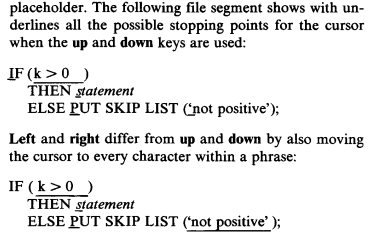
\includegraphics[width=0.4\textwidth]{img/cornell-ex.png}
    \end{multicols}
\end{frame}

\begin{frame}[hvid]
    \frametitle{Motivation and background (Continued)}

    \begin{multicols}{2}
        \begin{itemize}
            \item Hazel programming environment (2019)\footcite{omar}

        \end{itemize}

        \columnbreak
        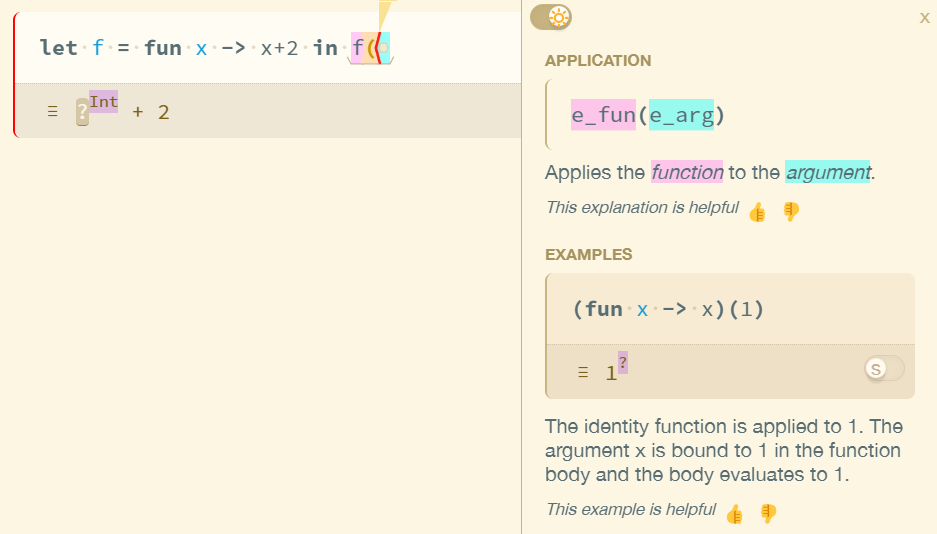
\includegraphics[width=0.5\textwidth]{img/hazel-ex.png}
    \end{multicols}
\end{frame}

\begin{frame}[hvid]
    \frametitle{Motivation and background (Continued)}

    \begin{multicols}{2}
        \begin{itemize}
            \item<1-> Type-Safe Structure Editor Calculus\footcite{godiksen}
            \item<2-> Implemented by a group of UCPH students\footcite{KU-bach}
            \item<3-> Generalized by a group of AAU students\footcite{aalborg}

        \end{itemize}

        \columnbreak
        \includegraphics<2->[width=0.5\textwidth]{img/ku-editor-ex.png}
    \end{multicols}
\end{frame}

\begin{frame}[hvid]
    \frametitle{Goal of the Project}
    \setbeamercovered{transparent}
    \begin{itemize}
        \item Implement an editor based on the generalized calculus
        \item Criteria for a good implementation:
              \begin{itemize}
                  \pause
                  \item Editing the abstract syntax of any program directly
                        \pause
                  \item Generic editing
                        \pause
                  \item Handling context-sensitive syntax
                        \pause
                  \item Multiple views of code being edited
                        \pause
                  \item Non-challenging way of specifying syntax
              \end{itemize}
    \end{itemize}
    \setbeamercovered{invisible}
\end{frame}

\begin{frame}[hvid]
    \frametitle{Related Work: Structure Editors}
    \begin{itemize}
        \item Cornell Program Synthesizer
        \item Hazel environment
    \end{itemize}
\end{frame}

\begin{frame}[hvid]
    \frametitle{Cornell Program Synthesizer}
    \begin{itemize}
        \item Overview
        \item Benefits and limitations
    \end{itemize}
\end{frame}

\begin{frame}[hvid]
    \frametitle{Hazel Environment}
    \begin{itemize}
        \item Typed holes and evaluation
        \item Feedback on incomplete programs
    \end{itemize}
\end{frame}

\begin{frame}[hvid]
    \frametitle{Related Work: Editor Generators}
    \begin{itemize}
        \item The Synthesizer Generator
        \item Centaur system
    \end{itemize}
\end{frame}

\begin{frame}[hvid]
    \frametitle{The Synthesizer Generator}
    \begin{itemize}
        \item Overview
        \item Attribute grammar specifications
    \end{itemize}
\end{frame}

\begin{frame}[hvid]
    \frametitle{Centaur System}
    \begin{itemize}
        \item Formalism in Metal language
        \item Maintaining syntactically correct trees
    \end{itemize}
\end{frame}

\begin{frame}[hvid]
    \frametitle{Related Work: Partial Evaluation}
    \begin{itemize}
        \item Program specialization
        \item Balancing generality and modularity
    \end{itemize}
\end{frame}

\begin{frame}[hvid]
    \frametitle{Program Specialization}
    \begin{itemize}
        \item General program and static input
        \item Specialized programs for performance
    \end{itemize}
\end{frame}

\begin{frame}[hvid]
    \frametitle{Balancing Generality and Modularity}
    \begin{itemize}
        \item Maintaining single program
        \item Specialization for different languages
    \end{itemize}
\end{frame}


\begin{frame}[hvid]
    \frametitle{Problem Statement}
    \begin{itemize}
        \item Edit abstract syntax directly
        \item Handle syntax of any language
        \item Context-sensitive syntax
        \item Multiple views of code
        \item User-friendly specification
    \end{itemize}
\end{frame}

\begin{frame}[hvid]
    \frametitle{Criteria for Solution}
    \begin{itemize}
        \item Direct editing of abstract syntax
        \item Generic handling of any language
    \end{itemize}
\end{frame}

\begin{frame}[hvid]
    \frametitle{Example Languages}
    \begin{itemize}
        \item C
        \item SQL
        \item LaTeX
    \end{itemize}
\end{frame}

\begin{frame}[hvid]
    \frametitle{Report Structure}
    \begin{itemize}
        \item Introduction
        \item Background
        \item Implementation
        \item Editor Examples
        \item Conclusion
    \end{itemize}
\end{frame}

\begin{frame}[hvid]
    \frametitle{Abstract Syntax}
    \begin{itemize}
        \item Abstract Syntax Trees (AST)
        \item Abstract Binding Trees (ABT)
    \end{itemize}
\end{frame}

\begin{frame}[hvid]
    \frametitle{Abstract Syntax Trees (AST)}
    \begin{itemize}
        \item Definition and purpose
        \item Example structures
    \end{itemize}
\end{frame}

\begin{frame}[hvid]
    \frametitle{Abstract Binding Trees (ABT)}
    \begin{itemize}
        \item Binding mechanisms
        \item Examples and benefits
    \end{itemize}
\end{frame}

\begin{frame}[hvid]
    \frametitle{Generalized Editor Calculus}
    \begin{itemize}
        \item Abstract syntax
        \item Semantics
        \item Encoding in extended $\lambda$-calculus
    \end{itemize}
\end{frame}

\begin{frame}[hvid]
    \frametitle{Abstract Syntax of the Editor Calculus}
    \begin{itemize}
        \item Sorts and operators
        \item Cursor and holes for every sort
    \end{itemize}
\end{frame}

\begin{frame}[hvid]
    \frametitle{Semantics of the Editor Calculus}
    \begin{itemize}
        \item Reduction rules
        \item Satisfaction rules
    \end{itemize}
\end{frame}

\begin{frame}[hvid]
    \frametitle{Encoding in Extended $\lambda$-calculus}
    \begin{itemize}
        \item Simply typed $\lambda$-calculus
        \item Encoding examples
    \end{itemize}
\end{frame}

\begin{frame}[hvid]
    \frametitle{Implementation Overview}
    \begin{itemize}
        \item Goals and criteria
        \item Tools and technologies used
    \end{itemize}
\end{frame}

\begin{frame}[hvid]
    \frametitle{Representing Syntax}
    \begin{itemize}
        \item Set of sorts
        \item Arity-indexed operators
        \item Sort-indexed variables
    \end{itemize}
\end{frame}

\begin{frame}[hvid]
    \frametitle{Syntax Representation}
    \begin{itemize}
        \item Definition of sorts and operators
        \item Example syntax representations
    \end{itemize}
\end{frame}

\begin{frame}[hvid]
    \frametitle{Code Generation vs Generic Model}
    \begin{itemize}
        \item Approaches to code generation
        \item Benefits and challenges of each approach
    \end{itemize}
\end{frame}

\begin{frame}[hvid]
    \frametitle{Generating Source Code}
    \begin{itemize}
        \item Parsing and syntax trees
        \item Code generation process
    \end{itemize}
\end{frame}

\begin{frame}[hvid]
    \frametitle{Parsing Syntax Trees}
    \begin{itemize}
        \item Parsing methods
        \item Examples and challenges
    \end{itemize}
\end{frame}

\begin{frame}[hvid]
    \frametitle{Source Code Generation}
    \begin{itemize}
        \item Tools and techniques
        \item Examples of generated code
    \end{itemize}
\end{frame}

\begin{frame}[hvid]
    \frametitle{Editor Expressions}
    \begin{itemize}
        \item Definition and usage
        \item Examples of editor expressions
    \end{itemize}
\end{frame}

\begin{frame}[hvid]
    \frametitle{Atomic Prefix Commands}
    \begin{itemize}
        \item Commands for tree traversal
        \item Examples and benefits
    \end{itemize}
\end{frame}

\begin{frame}[hvid]
    \frametitle{Conditional Expressions}
    \begin{itemize}
        \item Logical expressions for editor actions
        \item Examples of conditions
    \end{itemize}
\end{frame}

\begin{frame}[hvid]
    \frametitle{Editor Example: C}
    \begin{itemize}
        \item Syntax and operations
        \item Demonstration of editor functionalities
    \end{itemize}
\end{frame}

\begin{frame}[hvid]
    \frametitle{C: Syntax Representation}
    \begin{itemize}
        \item Definition of C syntax
        \item Examples and usage
    \end{itemize}
\end{frame}

\begin{frame}[hvid]
    \frametitle{C: Editor Operations}
    \begin{itemize}
        \item Editing operations in C
        \item Examples and benefits
    \end{itemize}
\end{frame}

\begin{frame}[hvid]
    \frametitle{Editor Example: SQL}
    \begin{itemize}
        \item Syntax and operations
        \item Demonstration of editor functionalities
    \end{itemize}
\end{frame}

\begin{frame}[hvid]
    \frametitle{SQL: Syntax Representation}
    \begin{itemize}
        \item Definition of SQL syntax
        \item Examples and usage
    \end{itemize}
\end{frame}

\begin{frame}[hvid]
    \frametitle{SQL: Editor Operations}
    \begin{itemize}
        \item Editing operations in SQL
        \item Examples and benefits
    \end{itemize}
\end{frame}

\begin{frame}[hvid]
    \frametitle{Editor Example: LaTeX}
    \begin{itemize}
        \item Syntax and operations
        \item Demonstration of editor functionalities
    \end{itemize}
\end{frame}

\begin{frame}[hvid]
    \frametitle{LaTeX: Syntax Representation}
    \begin{itemize}
        \item Definition of LaTeX syntax
        \item Examples and usage
    \end{itemize}
\end{frame}

\begin{frame}[hvid]
    \frametitle{LaTeX: Editor Operations}
    \begin{itemize}
        \item Editing operations in LaTeX
        \item Examples and benefits
    \end{itemize}
\end{frame}

\begin{frame}[hvid]
    \frametitle{Conclusion}
    \begin{itemize}
        \item Summary of findings
        \item Achievements of the project
    \end{itemize}
\end{frame}

\begin{frame}[hvid]
    \frametitle{Future Work}
    \begin{itemize}
        \item Implementation of missing editor expressions
        \item Multiple views and pretty-printing
        \item Integration with other languages
    \end{itemize}
\end{frame}

\begin{frame}[hvid]
    \frametitle{Future Directions}
    \begin{itemize}
        \item Extending the editor's capabilities
        \item Potential applications and improvements
    \end{itemize}
\end{frame}

\begin{frame}[hvid]
    \frametitle{Questions}
    \centering
    \large{Thank you for your attention!}
\end{frame}

\end{document}